%!TEX root = ../thesis.tex
%*******************************************************************************
%*********************************** First Chapter *****************************
%*******************************************************************************

\chapter{Introduction}  %Title of the First Chapter

\ifpdf
    \graphicspath{{Chapter1/Figs/Raster/}{Chapter1/Figs/PDF/}{Chapter1/Figs/}}
\else
    \graphicspath{{Chapter1/Figs/Vector/}{Chapter1/Figs/}}
\fi


\section{Introduction to epigenetics in prokaryotes, animals, and plants } %Section - 1.1 

Epigenetics refers to a “stably heritable phenotype resulting from changes in a chromosome without alterations in the DNA sequence” \cite{RN135}. In eukaryotic organisms, chromatin organisation plays a critical role in various cellular processes, including differentiation, development, response to environmental stimuli, and the maintenance of genome integrity. Chromatin consists of DNA and specialised proteins called histones, which together form nucleosomes. Histones exist in multiple variants and can undergo various modifications that influence chromatin structure, accessibility, and gene expression \cite{RN289,RN284}. The addition of a methyl group to the 5th carbon of cytosine results 5-methylcytosine (5mC) which is an example of DNA methylation - another epigenetic modification. In prokaryotic organisms, DNA methylation was originally identified as a component in the restriction-modification pathway wherein methylated sequences are recognised as self, and unmethylated sequences are targeted for cleavage by restriction enzymes, thus safeguarding the genome against invading unmethylated phage DNA \cite{RN96,RN95}.

In eukaryotic systems, including plants and animals, DNA methylation functions oppositely: invading transposable elements (TEs) are silenced by DNA methylation. In plants, 5mC is the most prevalent form of DNA methylation, primarily occurring in heterochromatic regions, though methylated loci can also be found in genic regions \cite{RN228,RN193}. DNA methylation can directly suppress transcription and gene expression by hindering the binding of transcription factors \cite{RN290}. One of the earliest evidences for epigenetic modifications in plants was discovered in the \textit{Arabidopsis thaliana} gene \textit{SUPERMAN} (\textit{SUP}). Mutations in \textit{SUPERMAN} affect normal floral development. Interestingly, some alleles exhibited the mutant phenotype without any alterations in the DNA sequence. The \textit{clark kent} epialleles were uncovered when it was discovered that the promoter sequence of \textit{SUP} was methylated. In addition, SUP expression correlates with the extent of \textit{SUP} promoter methylation \cite{RN100}. This discovery was among the first to highlight the role of DNA methylation in controlling transcriptional expression in plants. Since then, the field of plant epigenetics has significantly expanded, uncovering a myriad of complex mechanisms by which DNA methylation and other epigenetic modifications regulate gene expression, development and protect genome integrity throughout generations.

\section{Transposable elements} %Section - 1.2

The size of different plant genomes is highly variable and not necessarily related to their complexity. Among eukaryotes, flowering plants display the most extreme genome size variation, with differences of up to 2400-fold; for instance, the genome of \textit{Genlisea aurea} is just 63.6 megabases (Mb), while that of \textit{Paris japonica} reaches a staggering 150 gigabases (Gb) \cite{RN76,RN81}. TEs, which are selfish and repetitive DNA sequences, persist in genomes by copying and inserting themselves into various genomic locations \cite{RN102}. TEs are also essential for driving genome evolution: they can regulate gene expression, unequal crossover, recombination rate and in general contribute to genomic variation \cite{RN103}. TEs have had some prominent stabilising impacts on  chromosomes, playing a vital role in the evolution  of repetitive structures including the centromere  and telomeres \cite{RN101}.

However, the majority of TE activity tends to be harmful, posing risks to genome integrity and often being disadvantageous to the organism \cite{RN103}. Transposable elements can cause heritable disruption to a vast range of cellular functions by insertion into promoter, regulatory or genic regions. For example, the mobilisation of the \textit{CAC1} TE results in the disruption of the \textit{DWARF4}  gene and severe growth defects in \textit{Arabidopsis} \cite{RN105}.

TEs are categorized into two classes: Class I (retrotransposons) and Class II (DNA transposons) TEs. Class I TEs are transcribed via an RNA intermediate, which then undergoes reverse transcription before insertion at another site in the genome. The reverse transcriptase required for this process is usually encoded within the transposable element itself. One of the largest families of Class I TEs are long-terminal-repeat (LTR) retrotransposons. Some of these LTRs (flanking the TE) have acquired transfer-RNA (tRNA) fragments, which can be used as binding sites for host tRNAs. Subsequently, the clover leaf structure of the tRNA can be recognised as a primer to initiate reverse transcription and transposition. To combat this, some hosts cleave tRNAs into tRNA fragments (tRFs) that compete for these LTR binding sites, thereby silencing these retrotransposons \cite{RN66,RN67,RN68}.

Conversely, Class II TEs encode transposase enzymes that excise the DNA segments and insert them elsewhere in the genome.  Both Class I and Class II TEs can be further classified as either autonomous or non-autonomous elements. Autonomous elements encode all the necessary machinery for their own mobilisation, whereas non-autonomous elements lack some or all of these factors and rely on trans-acting transposases to facilitate their transposition \cite{RN106,RN107}.

In addition to disrupting the function of individual genes, the excision and insertion of TEs can destabilise genome structure \cite{RN103}. The repetitive nature of TEs can cause non-allelic homologous recombination during meiosis, leading to reproductive defects and the formation of dicentric or acentric chromosomes \cite{RN108}. 

The contribution of TEs to genome size varies massively: while they comprise only around 21\% of the \textit{Arabidopsis} genome \cite{RN109},  crops with larger genomes have gone through significant TE amplification typically dominated by a few TE families \cite{RN110,RN113}, resulting in an 82\% and 85\% genomic TE content of wheat and maize respectively \cite{RN110,RN111}. The importance of TEs in genome regulation is further exemplified in maize, where disruption of DDM1, a key chromatin remodeler required for the genome-wide maintenance of DNA methylation, results in embryo lethality \cite{RN112}. Thus, whilst mutations of the components of the pathway for establishment and maintenance of DNA methylation have no apparent phenotypic effects in \textit{Arabidopsis}, it offers an important model system for exploring the underlying mechanisms of genome-wide epigenetic regulation.

\section{Chromatin Structure}

The regulation of gene and TE transcription is essential for both prokaryotic and eukaryotic organisms. In eukaryotes, DNA is organised into chromatin, with the nucleosome serving as the basic unit. In a nucleosome, DNA is wrapped around histone octamers, which consist of two H2A-H2B heterodimers and one H3-H4 heterotetramer, along with the linker histone H1, altogether encompassing 147 base pairs of DNA \cite{RN294}. Nucleosomes are further organised into dynamic higher-order chromatin structures, which mediate chromatin accessibility and arrange the genome into more open, gene-rich euchromatic regions and more condensed heterochromatic regions, typically located around chromosome ends or pericentromeric regions in \textit{Arabidopsis} \cite{RN299}. 

Chromatin structure is regulated through histone modifications, such as acetylation, methylation, phosphorylation, or ubiquitination, which convey chromatin states and interact with various pathways that promote or repress chromatin accessibility and condensation.  For instance, trimethylation of lysine 27 of histone H3 (H3K27me3) and di- or trimethylation of lysine 9 on histone H3 (H3K9me2 or H3K9me3) are associated with repressed chromatin states. In contrast, H3K27 acetylation (H3K27ac) is associated with active promoters, as is histone H3 lysine 4 trimethylation (H3K4me3). Additionally, trimethylation of lysine 36 on histone H3 (H3K36me3) is correlated with active transcription in gene bodies \cite{RN297,RN298}. 

There are also specific histone variants that are either highly conserved across eukaryotes or unique to particular systems. For instance, H2A.Z is conserved across eukaryotes and is enriched in euchromatic regions, where it facilitates the recruitment of RNA Polymerase II in yeast, plants, and animals \cite{RN295,RN296}. In contrast, H2B.8 is specific to the sperm cells of \textit{Arabidopsis} and plays a key role in mediating sperm chromatin condensation \cite{RN285}.

\section{DNA methylation maintenance and the RdDM pathway} 

The existence of epigenetic marks implies that there are mechanisms to read, write and erase them. Cytosine methylation exists in one of three sequence contexts: the symmetric CG and CHG and the asymmetric CHH (where H = A, T or C).  This contrasts with mammals, in  which most methylation is directed to CG sites  and is not inherited by the next generation \cite{RN228}. 

\begin{figure}[htbp!] 
\centering    
    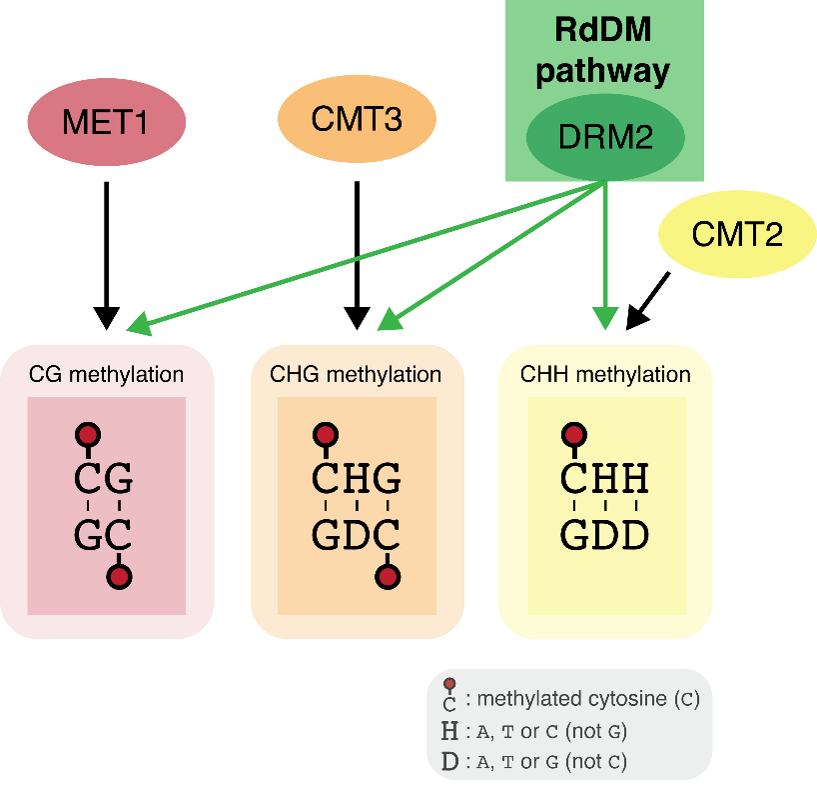
\includegraphics[width=0.5\textwidth]{Chapter1/Figs/base_mods.png}
\caption{DNA methylation sequence contexts and their associated DNA methyltransferases (Figure from \cite{RN61})}
\label{fig:meth_pathways}
\captionsetup{font=small}
    \caption*{}
\end{figure}

RNA-directed DNA methylation (RdDM) is a pathway that can methylate cytosine in any sequence context \cite{RN33}. In plants, it is also the only pathway responsible for the \textit{de novo} methylation of previously unmethylated regions. During DNA replication, modifications at symmetric CG and CHG sites result in a hemimethylated state, where only one strand of the daughter DNA retains methylation. Full methylation can be restored by the highly conserved maintenance methyltransferases METHYLTRANSFERASE 1 (MET1, a homolog of DNMT1) and CHROMOMETHYLASE 3 (CMT3) (Figure \ref{fig:meth_pathways}) \cite{RN61}. CHH sites are maintained by CMT2, however, due to the asymmetry of CHH methylation, methylation information may be lost during replication, necessitating the recruitment of RdDM for both \textit{de novo} methylation and maintenance. Therefore, to sustainably combat the detrimental effects of TE mobilisation, plants have evolved ways to keep transposon activity tightly controlled through RdDM. Additionally, the robustness of the system is enhanced by the fact that CMT2/3 and SET domain histone methyltransferases (KYP, SUVH5/6) maintain non-CG methylation and H3K9me2 in an interdependent manner. Specifically, the chromo and BAH domains of CMT3 interact directly with H3K9me2, allowing it to recognise other heterochromatic marks and establish a positive feedback loop \cite{RN33}.

Following the sequencing of the \textit{Arabidopsis} genome, two unexpected variants of RNA Polymerase II were discovered: RNA Polymerase IV (Pol IV) and RNA Polymerase V (Pol V) \cite{RN115}. Through these two variants, the RdDM pathway generates small RNAs (sRNAs) in heterochromatic regions and is able to target \textit{de novo} DNA methylation to these regions. The Pol IV-associated pathway initiates through recruitment via H3K9me2 associated chromatin remodeller SAWADEE HOMEODOMAIN HOMOLOG 1 (SHH1) \cite{RN206,RN98,RN99,RN116}.  Pol IV works in concert with chromatin remodellers CLASSY 1-4 (CLSY 1-4) to transcribe a short single-stranded RNA precursor \cite{RN117}, which is then extended into double-stranded RNA by RNA-dependent RNA polymerase 2 or 6 (RDR2 or RDR6) \cite{RN61,RN33}. This double-stranded RNA is processed by DICER-LIKE 3 (DCL3) into 24-nucleotide small interfering RNAs (24nt siRNAs), which are subsequently loaded onto specific ARGONAUTE proteins (AGO4/5/6/9) \cite{RN33} (Figure \ref{fig:RdDM_overview}). This complex interplay between DNA methylation and histone modifications ensures that patterns of DNA methylation are stably inherited through mitosis, maintaining consistent gene expression and genome stability across cell divisions.

\begin{figure}[htbp!] 
\centering    
    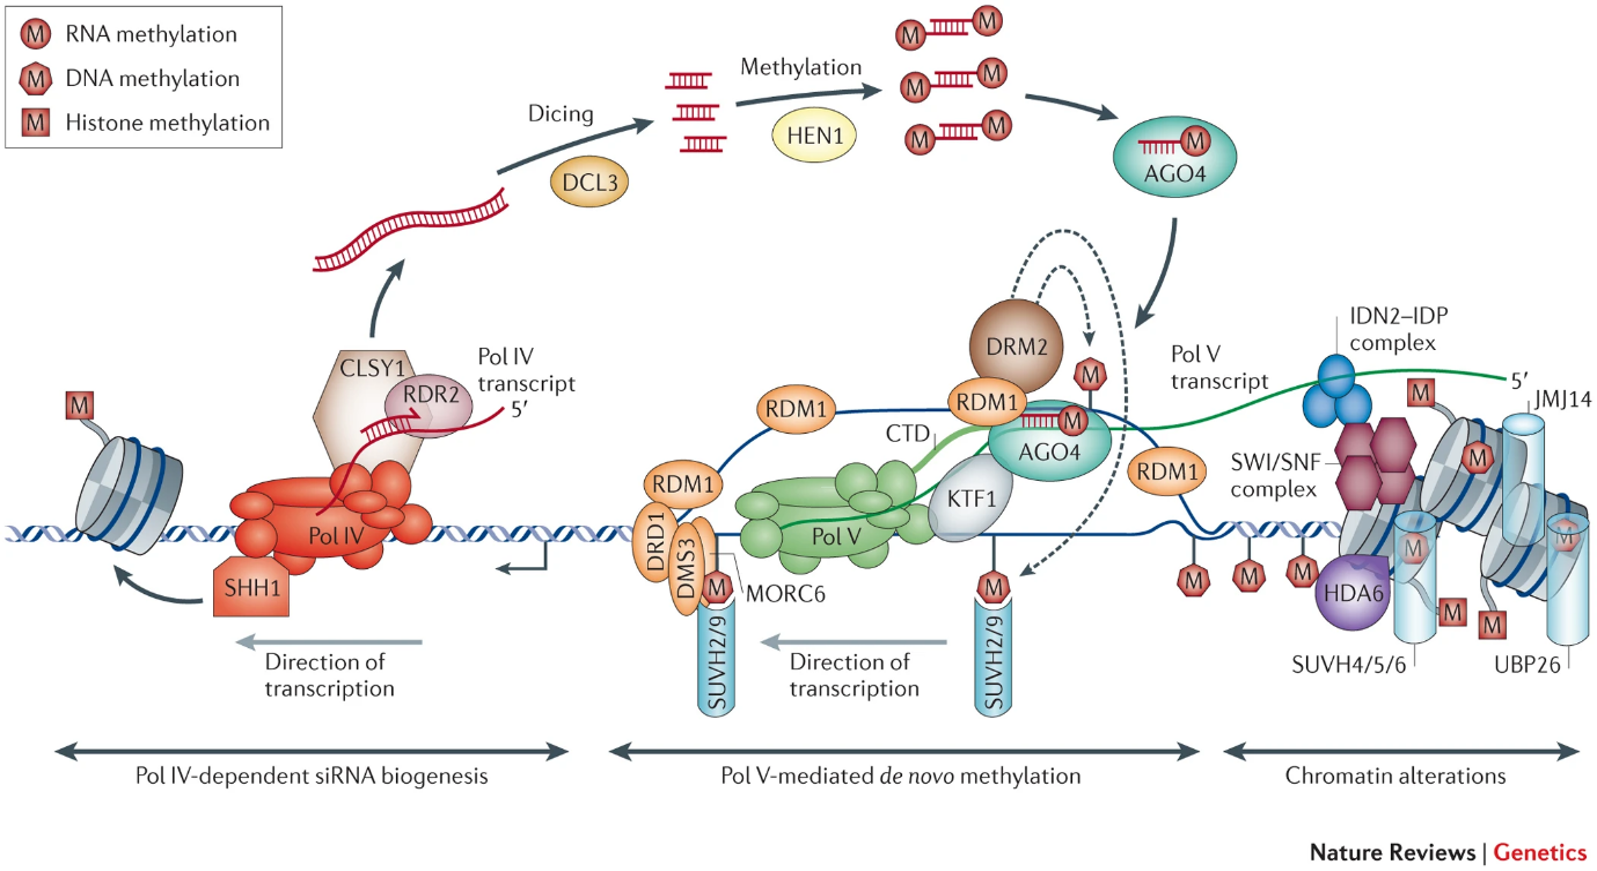
\includegraphics[width=1\textwidth]{Chapter1/Figs/RdDM.png}
\caption{An overview of the canonical RdDM pathway (Figure from \cite{RN33})}
\label{fig:RdDM_overview}
\captionsetup{font=small}
    \caption*{}
\end{figure}

Independently, Pol V is recruited by the DDR complex composed of chromatin remodellers DEFECTIVE IN MERISTEM SILENCING 3 (DMS3), DEFECTIVE IN RNA-DIRECTED DNA METHYLATION 1 (DRD1) and RNA-DIRECTED DNA METHYLATION (RDM1), along with SUPPRESSOR OF VARIEGATION 3–9 HOMOLOG 4/5/6 (SUVH4/5/6) methyl-DNA-binding proteins. The Pol V complex transcribes a single stranded RNA scaffold \cite{RN33}. The siRNA-AGO complex binds to this complementary scaffold RNA, and the AGO hook motif of the Pol V-associated SPT5-LIKE/KOW DOMAIN-CONTAINING TRANSCRIPTION FACTOR 1 (SPT5L/KTF1) protein subsequently binds to AGO4. NUCLEAR RNA POLYMERASE E 1 (NRPE1), the largest subunit of Pol V, and the \textit{de novo} methyltransferase DOMAINS REARRANGED METHYLTRANSFERASE 2 (DRM2) then associate with AGO4, catalysing DNA methylation (Figure \ref{fig:RdDM_overview})  \cite{RN228,RN121,RN122}. As discussed earlier, the maintenance of CHH sites depends on continuous \textit{de novo} methylation mediated by DRM2.

Recent studies have shown that the CLASSY (CLSY) family of chromatin remodelling factors regulates tissue-specific DNA methylation in \textit{Arabidopsis thaliana}, chiefly through the RdDM pathway. 5mC sequencing and sRNA sequencing across various somatic and germline tissues revealed distinct profiles of sRNAs and DNA methylation, driven by the tissue-specific expression of CLSY proteins. This provides a model where the unique expression profiles of chromatin remodellers shape tissue-specific DNA methylation \cite{RN162}.  


\section{Epigenetic reprogramming in plant sexual reproduction}

In mammals, primordial germ cells are sequestered early in development and go through genome-wide demethylation during development and following fertilisation. This results in the resetting of global epigenetic marks as well as restoring pluripotency \cite{RN210}. Subsequent \textit{de novo} re-methylation is mediated by methyltransferase Dnmt3 as well as germline specific PIWI-interacting small RNAs (piRNAs). The loss of the piRNA pathway results in transposon mobilisation, erroneous transcription regulation and reduction of fertility \cite{RN124,RN125,RN126}.

In the male lineage of angiosperms, the germline initiates from totipotent cells in the shoot apical meristem, giving rise to a diploid meiocyte. The meiocyte, surrounded by a layer of somatic nurse cells (the tapetum), undergoes meiosis, giving rise to a tetrad of microspores. The four microspores subsequently undergo mitotic division, to each make a vegetative cell (the somatic companion) and a generative cell, which divides further to make two sperm cells (Figure \ref{fig:male_sex_dev}) \cite{RN14,RN199} which forms the mature pollen grain. 

\begin{figure}[htbp!] 
\centering    
    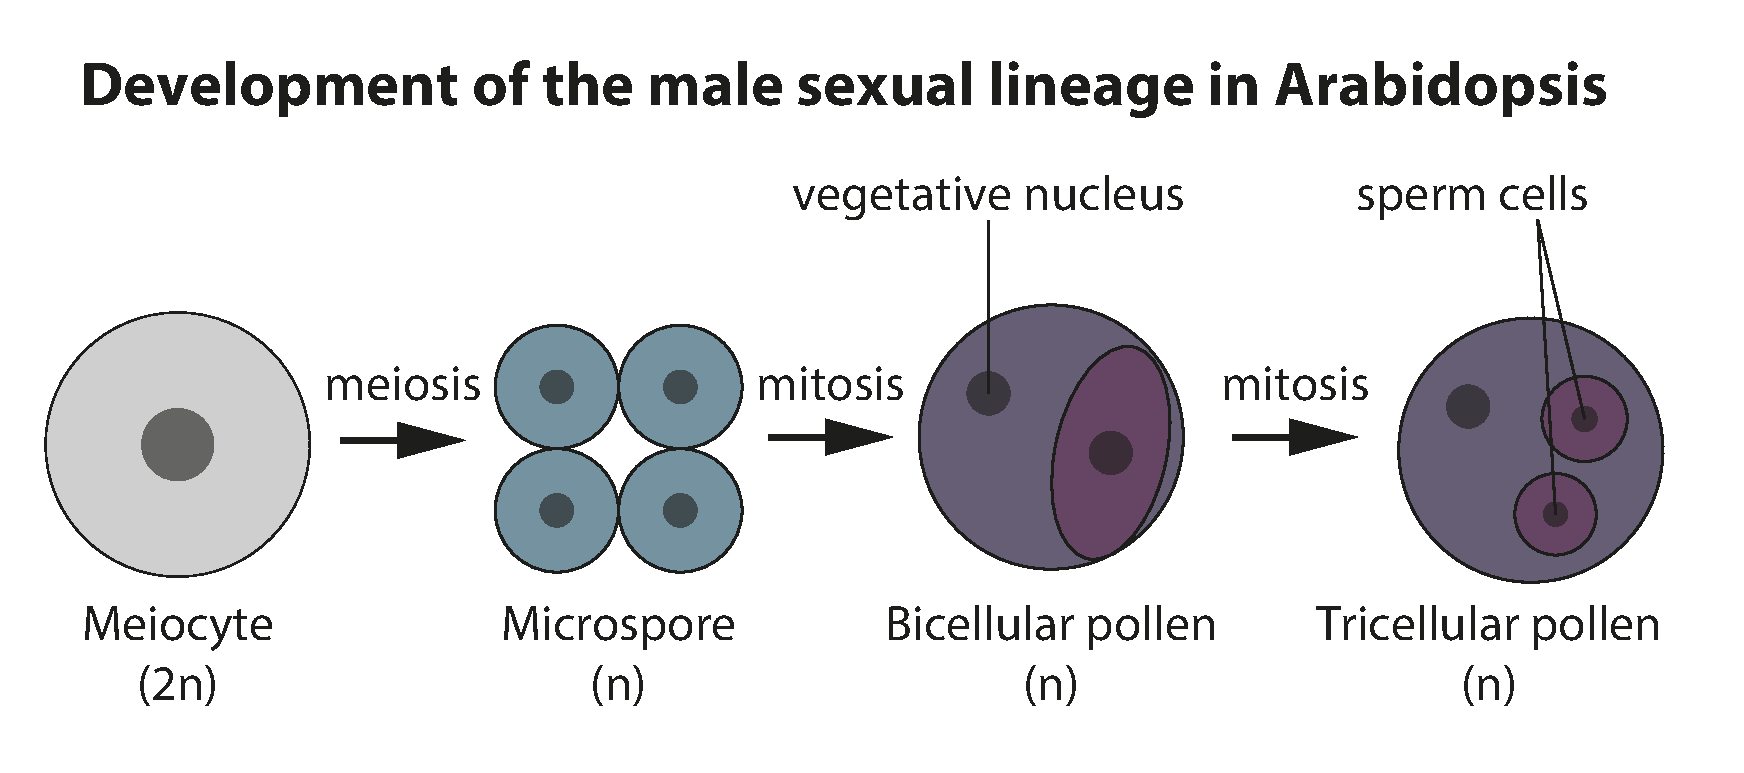
\includegraphics[width=1\textwidth]{Chapter1/Figs/male_sex_dev.pdf}
\caption{An overview of the development of the male sexual lineage in \textit{Arabidopsis}. Figure adapted from \cite{RN199}}
\label{fig:male_sex_dev}
\captionsetup{font=small}
    \caption*{\cite{RN199}}
\end{figure}

AGO proteins play crucial roles in sRNA pathways during reproduction. Recent findings have shown that during male meiosis, AGO1, AGO2, and AGO5 — proteins involved in post-transcriptional gene silencing (PTGS) — are localised in either the nucleus or cytoplasm, whereas AGO4 and AGO9 — associated with transcriptional gene silencing (TGS) — are found exclusively in the nucleus. \cite{RN149}. This study also provided an overview of the expression and localisation of several AGOs throughout meiosis, underscoring their dynamic expression and critical roles in germline development. Additionally, the presence of AGO1 and AGO5-bound micro RNAs (miRNAs) in meiocytes suggests that the miRNA pathway may be involved during meiosis \cite{RN149}. Furthermore, AGO5 and AGO9 have recently been shown to mark reproductive cells, similar to the early segregation of germline cells in animals \cite{RN291}. 

The RdDM pathway and sRNAs play crucial roles not only in germline development in \textit{Arabidopsis}, but also in other plant species. In maize, 21- and 24-nucleotide phased small interfering RNAs (phasiRNAs) are produced in the anthers and are essential for proper anther development \cite{RN292,RN293}. In sorghum, miRNAs were found to be differentially expressed before and after meiosis \cite{RN150}. In \textit{Arabidopsis}, cucumber, and soybean, several miRNAs are conserved and preferentially expressed in meiocytes, though their overall abundance is lower compared to somatic tissues \cite{RN151}. In rice, the ARGONAUTE protein OsAGO18 is specifically expressed in meiocytes, where it facilitates the accumulation of miRNA-triggered secondary siRNAs and regulates genes involved in pollen grain development \cite{RN153}. Additionally, the maintenance of CHH methylation through the RdDM pathway—particularly via RDR2, a critical component of RdDM—is necessary for both male and female sexual development in rice \cite{RN154}. Moreover, rice sporogenesis depends on the degradation of the germline-specific ARGONAUTE protein MEL1, which prevents off-target effects from rogue phasiRNAs; disruption of this process results in a semi-sterile phenotype \cite{RN155}.

Recent work identified male sexual lineage specific DNA methylation reprogramming in the \textit{Arabidopsis} germline, which will be discussed in detail in Chapter 2. Briefly, male meiocytes maintain high levels of CG and CHG methylation when compared to somatic canonical RdDM (cRdDM) loci levels, and a relatively low level of CHH methylation. However, in the CHH context, there is distinct hypermethylation at selected, sexual lineage specific loci (HyperTEs), including novel targets of RdDM activity. Additionally, \textit{de novo} gene-associated methylated loci (MetGenes) were also identified, including a meiosis-specific gene that was mis-spliced when methylation was disrupted \cite{RN199}. Recent evidence suggests that the biogenesis of these 24-nt sRNAs occurs in the somatic nurse cell layer surrounding the meiocytes, known as the tapetum \cite{RN187}. 

Similarly, in the female germline, the surrounding somatic tissue synthesises RNA polymerase IV-dependent 24-nt sRNAs from siren (siRNA in the endosperm) loci \cite{RN164,RN163,RN162}. Like the tapetal nurse cell-derived sRNAs that catalyse DNA methylation in male meiocytes, these siren loci-derived sRNAs are also dependent on CLSY3 and CLSY4 \cite{RN162}. However, there is little overlap between the loci targeted by these two sets of sRNAs, and even less between siren loci across different species \cite{RN163}. Despite their distinct origins, siren loci-derived sRNAs in \textit{Brassica rapa} similarly catalyse DNA methylation, predominantly at protein-coding genes, thereby regulating gene expression in the ovule \cite{RN165}. Furthermore, it has been recently shown that 24nt sRNAs accumulate in rice zygotes, which overlap gene rich, distinct loci from paternally derived sRNA loci \cite{RN166}, highlighting the conserved nature of 24 nucleotide sRNA driven DNA methylation reprogramming in both the male and female sexual lineage. The importance of RdDM in embryonic development is further underpinned by a recent study that showed embryos resulting from a maternal RdDM mutant cross result in incorrect gene expression in the endosperm and a reduction in seed viability \cite{RN167}.

\section{Thesis outline}

This thesis explores the dynamics of RdDM and DNA methylation after meiosis in the male sexual lineage of \textit{Arabidopsis} and in the embryo of \textit{Marchantia}.

In Chapter 2, the expression of CLSY chromatin remodellers, Pol IV, and Pol V in post-meiotic anthers of \textit{Arabidopsis} is investigated. This is followed by the sequencing and comparison of sRNA profiles from microspores, sperm cells, and sperm nuclei with other published germline and somatic datasets. Potential reactivation of sRNA biogenesis at cRdDM loci is revealed, and non-canonical RdDM pathways are implicated in sRNA biogenesis post-meiosis. Additionally, sRNA clusters derived from MetGenes and ATGP2N TEs in sperm cells are identified, along with a cluster of sperm-specific heterochromatic loci.

In Chapter 3, the sRNA and DNA methylation profiles of \textit{Marchantia} embryos are examined. MetGenes are defined in the sporophyte, and their connections to TE loci are identified. A method for isolating, imaging, and sequencing early embryos is tested, developed, and presented. Nuclear reporter lines are constructed to observe the phenotypic effects of knocking out paternal 4mC methylation in the embryo.

Each chapter contains a detailed materials and methods section, as well as appendices with supplemental information. In Chapter 4, the results are summarised in a broader context, and potential future directions, reflections, and limitations of the work are discussed.

